\documentclass[12pt,a4paper]{article}
\usepackage{graphicx}
\usepackage{caption}
\usepackage{natbib}
\usepackage{hyperref}
\usepackage{html}

\title{Limbic system map}
\author{Bernd Porr\footnote{BerndPorr@glasgow.ac.uk}, Maria Thomson and Ailsa Millen}
\date{Version \input{tag.txt}}

\begin{document}


\maketitle

\begin{latexonly}
\begin{figure}[!htb]
    \begin{center}
    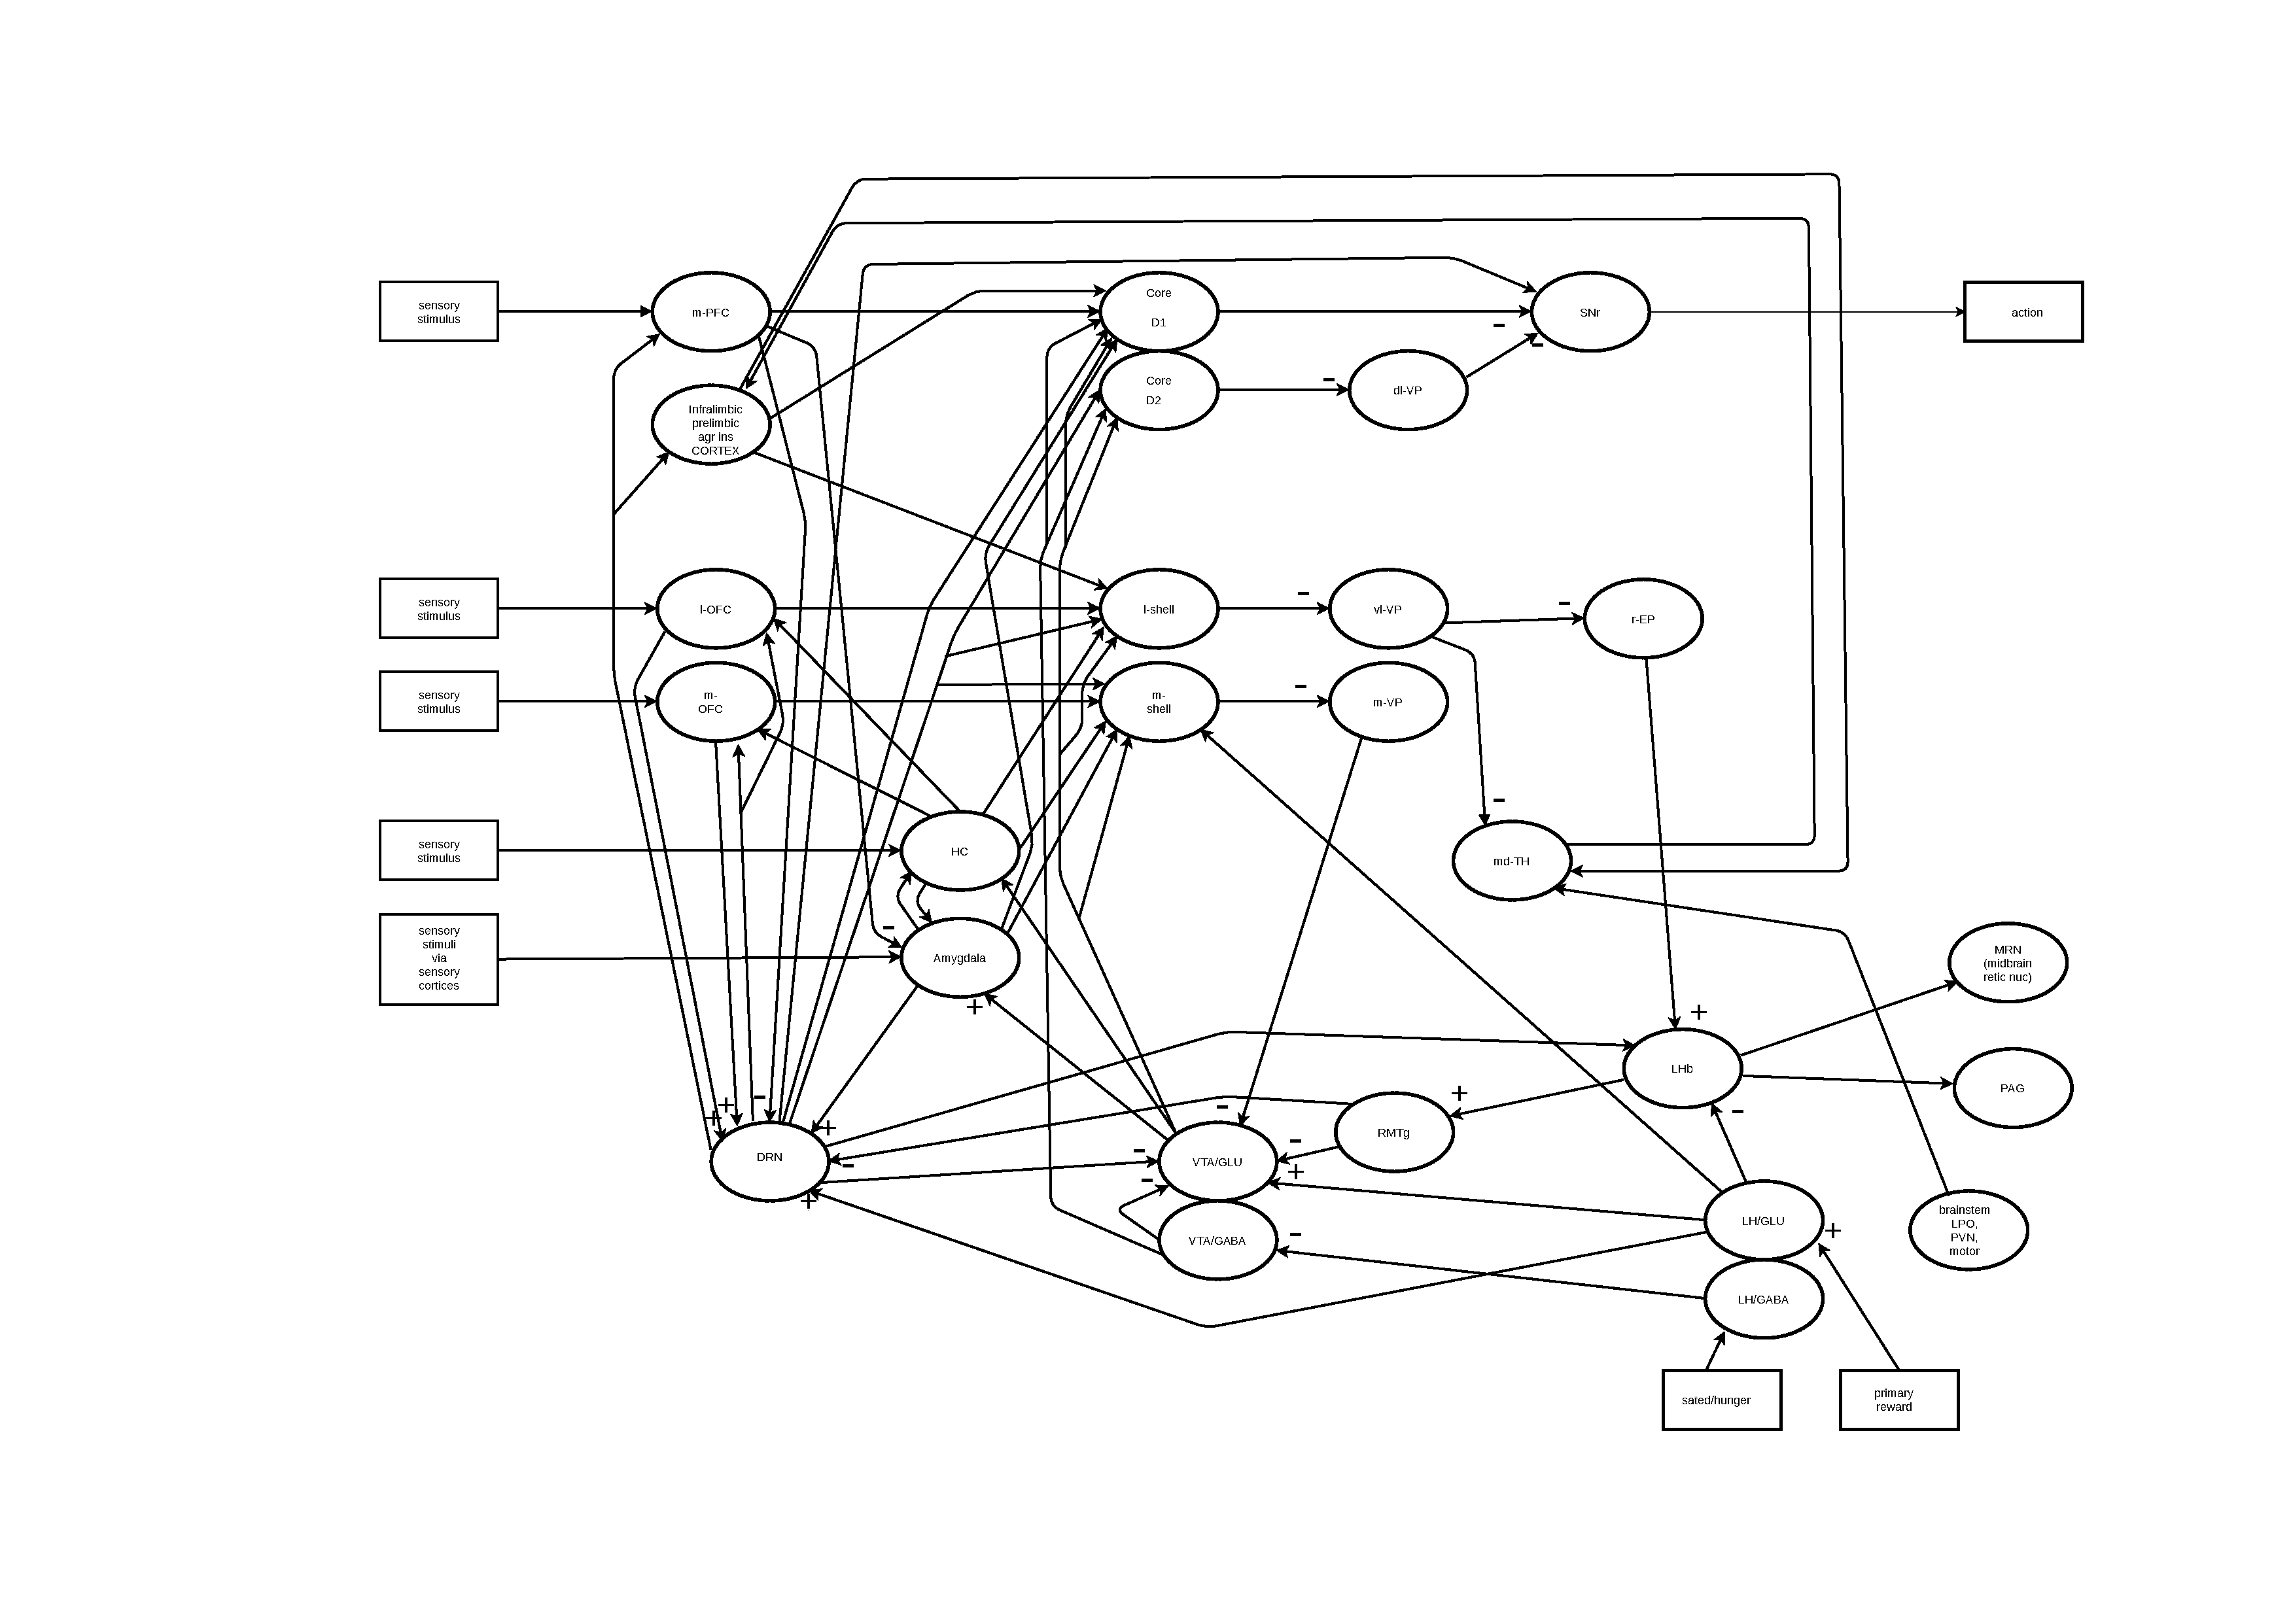
\includegraphics[width=\textwidth]{limbic-map}
    \end{center}
\end{figure}
\end{latexonly}



\tableofcontents

\section{Introduction}
This page is a hybrid of a map and a explanations underneath underneath which in turn points to references which back up the connections.

The main aim is to have a map of the limbic system which is supported by references which then in turn can inform computer models which simulate behavioural experiments.




\subsection{Review articles}
\begin{itemize}
\item This article by Castro and Berridge promotes their long standing differentiation between 'wanting' and 'liking' \citep{Berridge2009} now updated by 'hedonic hot spots' \citep{Castro2015}.
\item Berthoud's article features fantastic connection diagrams between the different nuclei of the limbic system \citep{Berthoud04}.
\item Zahm again provides very detailed anatomical connection diagrams and is a must read \citep{Zahm00}.
\item The review by  Abbas Khani and Gregor Rainer focusses on the roles of the different nuclei, how they interact, how they implement reinforcement guided decision making and which forms are out there (reversal, go no go etc). A very balanced article which, for example, not just cites the prediction error paradigm of DA but reports also the other roles DA \citep{Khani2016}.
\end{itemize}










\section{Amygdala}

The connectivity of the amygdala has been outlined in these reviews \citep{Alheid2003}, \citep{Sah2003} and \citep{Swanson1998}.

\subsection{Central / Medial}

For the  the central and medial Amygdala \citep{Swanson2003}\citep{Swanson1998} have pointed out that these parts contain cells which are similar to those in the striatum (i.e. GABAergic) and thus can be seen as an extension of the striatum dealing with lower executive or autonomic functions.

\subsection{Basolateral / lateral}

The basolateral part of the Amygdala which is related to reward processing and has glutamatergic neurons which have similar roles to that of the cortex and then projects into the striatal parts of the amygdala. See Fig 5 and 6 in \citep{Swanson1998} for very informative connection diagrams.

\subsection{Efferents}

The anterior basolateral amygdala projects to the NAcc core and the  posterior part to the extended amygdala structures  \citep{Alheid2003}.

A projection from the Amygdala to the DRN \citep{PollakDorocic2014} has been reported.

\subsection{Afferents}

The basolateral Amygdala has abundant projections from somatosensory cortices 
\citep{Swanson1998}, limbic cortices \citep{Ottersen1982} and (ventral) hippocampus \citep{Pitkanen2000}.

mPFC inputs are inhibitory in nature \citep{Rosenkranz2002} but this inhibition can be suppressed by DA release so that in the presence of DA the cortex can drive the BLA.




\section{Dorsal Raphe Nucleus (DRN)}

Review papers by Michelsen and Schmitz \citep{Michelsen2007} and \citep{Nakamura2013}.

The DRN seems to generate 5HT to “wait to obtain a reward” behaviour  \citep{Nakamura2013}.

\subsection{Afferents}

A detailed tracing / optogenetic study can be found here  \citep{PollakDorocic2014}.

LHb, mPFC and LH appear to be the main afferents to the DRN \citep{Vertes2010} \citep{Sparta2014} \citep{Lee2003}.

\subsubsection{OFC to DRN}

The OFC has strong reciprocal connections to with DRN \citep{Zhou2015} where the OFC is probably the main nucleus of the DRN's ability to track the long term anticipated reward and reversal learning \citep{Roberts2011}.

\subsubsection{mPFC to DRN}

The mPFC (in particular its ventral part) has GLU projections to the DRN \citep{Goncalves2009} \citep{Lee2003}.

The conventional view is that the mPFC’s glutamergic projections to the DRN connect to locally inhibitory neurons that then target 5HT neurons \citep{Celada2001}. Stimulation of mPFC neurons usually inhibit DRN neurons which makes a strong case for these scenario.

However, \citep{PollakDorocic2014} found that the mPFC has direct excitatory control of 5HT which they consider to be potentially critical for the correct function of the serotonergic system. 

\subsubsection{LHb to DRN}

Similarly with regards to LHb projections to the DRN the conventional view is that the LHb neurons
target local GABA neurons that then inhibit 5HT. However, \citep{PollakDorocic2014} found a direct connection to the DRN. Contrary to \citep{PollakDorocic2014}, \citep{Ogawa2014} found few monosynaptic connections from the LHb to the DRN and instead posits that the LHb inhibits DRN 5HT via the rostral medial tegmental nucleus (RMTg). This has also been confirmed by \citep{Sego2014}.

Overall the picture emerges that the LHb exerts its influence via the RMTg and that direct connections from the LHb to the DRN are rare.

\subsubsection{LH to DRN}

Strong monosynaptic glutamatergic projections have been shown by \citep{Lee2003} and \citep{Aghajanian1990}. It's interesting that of these most prominent projections mentioned above it appears that this is the only excitatory one.

\subsubsection{Amygdala to DRN}

Tracing studies have shown robust projections from the Amygdala (CEA) to the DRN \citep{PollakDorocic2014} which are monosynaptic and are most likely glutamatergic \citep{Swanson1998}. In contrast to the GABAergic inputs above this seems to be one of the few excitatory inputs.

\subsubsection{Basal Ganglia to DRN}

Several nuclei from the basal ganglia project to the DRN including SNr and globus pallidus which is inhibitory in nature \citep{PollakDorocic2014}.

\subsubsection{Anterior cingulate cortex (ACA)}

The paper by  \citep{PollakDorocic2014} has also shown an excitatory pathway from the ACA to the DR.

\subsection{Efferents}

Most recently the projections to the limbic cortices have been identified as the strongest \citep{Linley2013} \citep{Roberts2011} whereas in this older publication \citep{Reisine1984} states that the DRN projects to the striatum and caudate nucleus. 

The paper by \citep{Vertes2010} claims the DRN efferents include the VTA, SNc, LH and NAcc core. \citep{Nakamura2013} stresses the projections from the DRN to the SNr, the VTA (inhibitory), amygdala, cortex (with inhibition of the mPFC) and to the NAcc where 5HT has at least partially a disinhibitory effect by targeting interneurons.

The actual effect of 5HT depends on the prominent receptor type in the target area. Some 5HT receptors are excitatory, some inhibibitory and some ramp up plasticity \citep{Frazer1999}.

The review paper by \citep{Michelsen2007} makes a distinction between dorsal, medial and ventral pathways:

\subsubsection{Dorsal pathway of the DRN}

  * all parts of the striatum ranging from the Nacc shell over core to the dorsal striatum
  * to a lesser extent the globus pallidus (GP)

\subsubsection{Medial pathway of the DRN}

  * mainly the SNr.

\subsubsection{Ventral pathway of the DRN}

This pathway targets a large number of different limbic nuclei. In order of density:

  * Septum (dense)
  * Amygdala (dense)
  * Habenula (dense)
  * Piriform, insular and frontal cortices (dense)
  * Occipital, entorhinal, perirhinal, frontal orbital, anterior cingulate and infralimbic cortices (moderate)
  * Thalamic and hypothalamic nuclei (dense to moderate)
  * Olfactory bulb. \citep{Lottem2016} has shown that the spontaneous activity of the olfactory cortex is suppressed by 5HT release but that odor evoked activity is unaffacted by 5HT.
  * Hippocampus
  * Interpeduncular nucleus
  * Geniculate body


\subsection{Receptors}

In contrast to dopamine 5HT has a vast array of different receptors. While the DRN and MRN generate a global 5HT signal the effects on different brains areas can be vastly different because of every brain area has their own 5HT receptor distribution \citep{Palacios1990} \citep{Carhart-Harris2017}. Before we go into the efferents we present the different receptors and where they are located. If not otherwise cited it's based on the review by \citep{Mengod2010} and the classic \citep{Palacios1990}.

\subsubsection{5HTR1}

The 5HTR1 has numerous subclasses:
  * 5HTR1A receptors are found on excitatory/pyramidal neurons and inhibit those. This receptor has been called the "limbic" receptor because it is prominent in the limbic areas of the brain: hippocampus, lateral septum, cortex (cingulate/entorhinal) and raphe nucleus. These receptors are often co-expressed with the excitatory 5HT2A receptor. They are located on the soma or dendrite and thus can inhibit the firing of neurons \citep{Riad2000}.
  * 5HTR1B are found mainly on inhibitory neurons and inhibit those but occasionally also on pyramidal neurons. They are very prominent in the basal ganglia, in particular in the GP, SNR, VP and EP (which are the output nuclei of the BG). They are both auto and heterosynaptic receptors and are located at the axon terminals \citep{Riad2000} and control rather the release of transmitter in contrast to 5HTR1A which control spiking.
  * 5HTR1D are located in the caudate putamen, Nacc, olfactory cortex, dorsal raphe nucleus und locus coeruleus. It's predominantly located on axon terminals of both 5HT and and non 5HT neurons and inhibit release of neurotransmitters.
  * 5HTR1E is prominent in the (entorhinal) cortex, caudate putamen and claustrum.
  * 5HTR1F has its highest levels in the cortical regions, olfactory bulb, Nacc, parascicular nucleus, thalamus, medial mamillary nucleus, hippocampus, subiculum and amygdala.

Having both inhibitory 5HT receptors on both excitatory and inhibitory neurons means that this can cancel out in average but will possibly change the dynamics of the network.

\subsubsection{5HTR2}

  * 5HTR2A: These receptors are excitatory and enhancing inputs when activated meaning they are located on dendrites and on the soma. These receptors are very prominent in the cortex and have been localised on GABAergic interneurons but also glutamatergic projection neurons.
  * 5HTR2B: it's function and localisation is still poorly understood
  * 5HTR2C: has only been found in the CNS and there in the choroid plexus, cortex, NAcc, hippocampus, amygdala, caudate and SNr. They are also postsynaptic but might be also presynaptic.

\subsubsection{5HTR3}

It's highest concentration is in the dorsal vagal complex of the brainstem. 

Is a fast excitatory receptor which is mainly located in the hippocampus (and possibly amygdala) \citep{Palacios1990} and is co-expressed with GLU receptors in the hippocampus.

Some evidence points to it controlling DA release \citep{Mengod2010}.

\subsubsection{5HTR4}

This receptor seems to control primarily plasticity, for both LTP and LTD \citep{Penas-Cazorla2015}. In an experiment by \citep{Mlinar2006} stimulation of this receptor causes LTP in hippocampal slices which were very long lasting for over 2hrs.

Even more impressive are the findings by \citep{Hagena2017} who show that 5HTR4 activation shifts the frequency threshold between LTD and LTP: it is generally accepted that under LFS LTD is induced whereas under HFS LTP is induced. The frequency threshold where LTD turns into LTP can be shifted by the 5HTR4 receptor. If this receptor is stimulated even lower frequencies can cause LTP which otherwise would have caused LTD!

In the rat it is located mainly in the limbic system: hippocampus, striatum, inferior colliculus, SNr, ventral pallidum, fundus striatae, olfactory tubercle, septum and amygdala. It has also high concentrations in the parietal cortex.




\subsection{Activity}

As shown by \citep{Li2016}: the activity increases when "when a mouse voluntarily seeks and acquires sucrose, food, sex and social interaction". 5HT neurons are activated by surprising reward events (such as VTA neurons do) and reward predicting cues is presented. The activity only drops off after the reward has been experienced. In particular the DRN activity stays active while the animal is waiting for a reward.

\subsection{Behavioural studies}

Numerous studies have reported that 5HT is required for delayed reward scenarios, for example where a rat has to wait in front of a dispenser to retrieve a reward \citep{Khani2016} as already mentioned above where the activity was measured during a delayed reward scenario \citep{Li2016}.

This has been combined into the proposal by \citep{Miyazaki2012} that 5HT controls patience and reward.

Premature responding is increased after \citep{Fletcher2007} application of a 5HT(2A) receptor antagonist and decreased after 5-HT(2C) application. In earlier studies impulsivity could also be increased by 5HT depletion \citep{Harrison1997}.







\section{Entopeduncular Nucleus (EP)}

The entopeduncular nucleus’, also called the GPi in primates, actions are
strongly regulated by expected reward outcomes and it is an important output centre of the basal ganglia \citep{Rajakumar1993} 

\subsection{Efferents}

Different parts of the EP appear to perform different tasks. 

  * The caudal part of the EP has efferents to the (vm-)thalamus and brainstem nuclei and therefore controls motor activity \citep{Rajakumar1993}  \citep{Wallace2017}.
  * The rostral part of the EP has strong projections to the lateral subnuclei of the LHb (including the oval nucleus)LHb \citep{Rajakumar1993}\citep{Hong2008} which are glutamatergic and excitatory \citep{Shabel2012} \citep{Wallace2017}. The LHb then projects primarily to the rostral medial tegmental area (rMTg) which is a GABAergic nucleus that innervates the VTA.

\subsection{Function}

The reward prediction error is considered to be instigated from the LHb and Barrot et al, 2012 theorized that the EP could play a major role in this activity as it has such an important input to the LHb \citep{Barrot2012} and in turn to the VTA as menioned above. This relates to the rostral part of the EP.







\section{Lateral Habenula}

\subsection{Afferents}

The 2 strongest forebrain afferents to the LHb are the EP and LH and other connections include the lateral preoptic area and the VP \citep{Parent1981}. 

Araki, 1984, states that the connection from EP to LHb is GABAergic \citep{Araki1984} but Shabel 2012 qualifies it as excitatory and glutamergic \citep{Shabel2012}.

Mok proposed that the actual connection was mainly excitatory \citep{Mok1974}. A view supported by Poller who found a strong glutamergic projection that targeted VTA and RMTg projecting neurons \citep{Poller2013}.

The LHb also receives DA input from the midbrain VTA and SNc \citep{Kowski2009} and reciprocally its main, inhibitory projections are to the VTA, SNc and the DRN \citep{Ji2007}\citep{Christoph1986}\citep{Rajakumar1993}.

\subsection{Efferents}

The main targets of the LHb are the VTA, Midbrain reticular nucleus (MRN), periaqueductal gray (PAG) and the superior central nucleus raphe (CS) \citep{Quina2015}.

Slightly puzzling is that the effect on the VTA by the LHb is known to be inhibitory. Hong et al’s 2011 theorize that as LHb neurons are largely glutamergic their inhibitory function must be through an intermediary, the RMTg \citep{Hong2011}.

\subsection{Function}

Bromberg-Martin et al’s 2010 research viewed LHb as the most important source of reward memory in DA neurons. They cited 3 potential pathways for transmission; 1) prefrontal cortex to the striatum to the global pallidus to LHb 2) For rats, the mPFC to LHb 3) common sources project reward memory signals to LHb and DA neurons. They found that many LHb and DA neurons signalled past reward results in their tonic activity, this was surprising as previous studies had reported this was purely the case for phasic activity \citep{Bromberg-Martin2010}.

It is considered to be the main source of the negative reward signal that facilitates the DA reward prediction error as LHb innervation inhibits midbrain DA.\citep{Shen2012}\citep{Shabel2012}\citep{Matsumoto2007}\citep{Barrot2012} 





\section{Lateral hypothalamus (LH)}

The lateral hypothalamus has both Glutamatergic and GABAerfic neurons \citep{Stanley2011}.

\subsection{Efferents}

The strongest outputs from the LH are to the VTA and the lateral habenula (LHb) \citep{Stuber2016}. 
The projection from the LH to the Habenula is excitatory \citep{Poller2013} which in turn then projects to the RMTg which has GABA-ergic neurons.

The LH contains both Glu and GABA neurons where the GLU neurons project to the DA neurons in the VTA whereas the GABA neurons in the LH project to the GABA neurons in the VTA which in turn then disinhibit DA neurons in the VTA. 


\subsection{Afferents}

The LH receives many different inputs from different cortical and subcorical areas which are both excitatory and inhibitory. The PFC seems to be an import source of excitatory information, in particular the mPFC. It also receives inputs from the extended Amygdala and the hippocampus \citep{Stuber2016}.

\subsection{Behavioural experiments}

Feeding is stimulated when LH cells are activated by glutamate
agonists \citep{stanley93} and that stimulation of GABAergic cells in the LH inhibits feeding \citep{Stanley2011}.





\section{Nucleus Accumbens Core}

\subsection{Afferents}

The NAc core receives inputs from the dorsal-medial prefrontal cortex and the hippocampus \citep{brog93}.

\subsection{Efferents}

There are two distinct output pathways from the NAcc core which have its origins from the two sub-populations of neurons in the NAcc core. The one sub-population carries mainly D1 receptors and the other one carries mainly D2 receptors \citep{kelley04} \citep{Humphries2010}. 

\subsubsection{Direct pathway}

The D1 receptor carrying neurons feed directly into the SNr and are able to inhibit tonically active SNr neurons, thus the NAcc core is able to disinhibit motor programs. 

\subsubsection{Indirect pathway}

There is an indirect pathway via the VP to the SNr originating from the NAcc core. In contrast to the direct pathway these neurons in the indirect pathway carry mainly D2 receptors which are inhibitory in nature. D2 receptors are very sensitive to low DA concentrations and will react to the tonic DA concentrations. 




\section{Nucleus Accumbens Shell}

The shell can be further divided into the medial and lateral shell \citep{Ikemoto2007} \citep{Usuda1998} used in the model by \citep{Humphries2010}.

\subsection{Medial Shell}

The medial Shell projects to the medial Ventral Pallidum (VP) \citep{Ikemoto2007}.

\subsection{Lateral Shell}

The lateral shall projects to the ventrolateral Ventral Pallium (VP) \citep{Ikemoto2007}.


\subsection{Behavioural experiments}

The shell seems to be responsible for behavioural flexibility meaning that it controls the animal's ability to shift to another target when the reward is lost \citep{Aquili2014}

\subsection{Function}

Overall the Shell seems to learn the stimuli which are associated with a reward, and thus enhances the future salience of those stimuli \citep{Cassidy2017}.

In this context it is also interesting that shell DA also tracks rather the inventive value than the reward prediction error \citep{Sackett2017} which probably means that the VTA has regions which work with the shell and that they are distinct from the core.




\section{Nucleus Accumbens (NAcc)}

The Nacc is the ventral extension of the striatum, and therefore also called the ventral striatum.  The ventral striatum contains neurons known as medium spiny neurons (MSN's).

The accumbens has two major subterritories: the shell and the core 
\citep{heimer91} where the shell can be further subdivided \citep{Usuda1998} in lateral and medial parts and the core rather depending on its D1 or D2 receptors.

[[nacc-shell]]

[[nacc-core]]

\subsection{Behavioural experiments}

The Nacc core and shell have distinct roles controlling reward based learning:

In reversal learning \citep{Dalton2014} the shell seems to control switching contingencies (i.e. the reward is moved from one site to another) whereas the core controls the actual approach behaviour towards the rewarding site.

Impulsivity is altered by 5HT antagonists which point towards an important role of 5HT in the retrieval of delayed rewards. 5-HT(2A) antagonists reduced decreased impulsive responding and the 5-HT(2C) antagonist increased impulsivity \citep{Robinson2008}.

\subsection{Signals}

By measuring the DA concentration in both the core and shell \citep{Saddoris2015} it turns out that Core DA follows the classical prediction error signals were it spikes most to the predicting cue whereas the shell responds to all reward related events during the experiment.

\subsection{Plasticity}

It's well known the bursts of dopamine cause LTP in conjunction with pre- and (possible) postsynpatic activity (so called 3 factor Hebbian rule) or heterosynaptic LTP. However \citep{Goto2005} showed that D1 receptors cause LTP on hippocampal fibres whereas D2 receptors control the cortical inputs in the opposite way.
It appears to be that 5HT causes retrograde cannabinoid (CB) release which inhibits pre-synaptic GLU release \citep{Burattini2014}. However, also postsynaptic HFS causes CB1 mediated depression. \citep{Mathur2011} tested this more thoroughly in that they conclude that 5HT actually causes presynaptic inhibition via the 5HT1B receptor, with that LTD and that HFS can have a similar effect by releasing CB.



\section{Orbitofrontal Cortex (OFC)}

The OFC associates sensory stimuli with reward related information \citep{Schoenbaum.2009} or in other words it computes the (potential) reward value of a sensor cue \citep{Wikenheiser2016}, \citep{Bari2013}.

\subsection{Afferents}

The OFC receives inputs from a wide range of brain areas which allows it associate sensor cues (and also actions) to rewards. \citep{Wikenheiser2016} provides an overview of these inputs which are from the:

\begin{itemize}
\item hippocampus
\item subiculum
\item PFC
\item perihirnal cortex, and
\item nucleus reuniens
\end{itemize}

Serotonin seems to have a strong effect on the OFC which has been shown by \citep{Zhou2015}. Stimulation of the DRN results in both excitatory activity and inhibitory activity in the OFC. In addition the release of 5HT has a strong impact on plasticity: after pairing an odour stimulus with the release of 5HT the odour stimulus creates long lasting activity in the OFC which starts at the presentation of the stimulus and ends after reward delivery  \citep{Zhou2015}.

\subsection{Efferents}

Its major subcortical targets include the dorsal raphe nucleus \citep{Luo2015}, medial striatum, NAcc, lateral preoptic area, amygdala and the hypothalamus \citep{Vertes2012}.

  * The l-OFC innervates the l-shell and amygdala and 
  * the mOFC the m-shell, hippocampus and amygdala \citep{Brog1993} \citep{Noonan2012}

\subsection{Neuronal activity}

The paper by \citep{Tremblay1999} proposed that OFC neurons code the motivational value of rewards. The activity of OFC neurons increased in response to reward-predicting stimuli, during the expectation of rewards, and after the receipt of rewards. Also actions, associated with rewards, increase the firing rates of OFC neurons \citep{Wikenheiser2016}.

\subsection{Behavioural experiments}

The review by \citep{Wikenheiser2016} presents behavioural experiments involving the OFC which confirm that the OFC computes behavioural reward value computed from sensory cues, such as odour, and actions. They contrast this to the hippocampus which computes reward value in relation to place fields.

Spatial reversal learning is improved by injecting the 5-HT(2C) receptor antagonist into the OFC \citep{Boulougouris2010}. 

Reversal learning is impaired if 5HT processing is disrupted in the OFC \citep{Bari2013}.

\subsubsection{Medial Prefrontal Cortex (mPFC)}

The mPFC is considered by Homberg to be the most important location for top level cognitive
functions. 

The ventral portion of the mPFC is called Infralimbic cortex (IL) \citep{Tsutsui-Kimura2016}.

\subsection{Efferents}

A well known target of the mPFC is the Nacc core where the Nacc seems to be taking the role for response inhibition and waiting \citep{Neufang2016} \citep{Feja2014}.

Projections from the mPFC to the DRN, allowing the mPFC to regulate 5HT firing and therefore control its own 5HT innervation  \citep{Homberg2012}\citep{Juckel1999}. This projection is inhibitory (see also the DRN page).

\subsection{Neuromodulation}

5HT plays a significant role in the mPFC which has been shown in great detail in \citep{Santana2017} and concluded that 5-HT1A, 5-HT2A, 5-HT2C, and 5-HT3, 
dopamine D1 and D2 are widely expressed in the mPFC. The receptor 5-HT3 was only expressed on GABAergic interneurons while all the other ones were expressed on both pyramidal and interneurons.


\subsection{Behaviour}
Lesions to the IL causes more impulsive behaviour \citep{Tsutsui-Kimura2016} and reduction in 5HT is also associated with less impulse control \citep{Neufang2016}.



\section{Rostral Medial Tegmental Nucleus (RMTg) }

The newly discovered rostral medial tegmental nucleus, also called the tail of
the VTA, is partially embedded in the VTA \citep{Bourdy2012}. It has been suggested that it has
an ideal location to function as a switch between opposing aversion and reward
responding areas and to direct information to DA neurons \citep{Barrot2012}.

\subsection{Afferents}

The main afferent to the RMTg is the glutamergic connection from the LHb, which is 7 times
stronger than the LHb projection to the VTA \citep{Barrot2012} and other afferents include
the VTA and SNc \citep{Lavezzi2011}.

RMTg GABA neurons differ in their targets to the VTA GABA neurons which, for example, target the forebrain in large numbers \citep{Barrot2012}. 

\subsection{Efferents}

The RMTg’s GABA efferents are the principal inhibitory connection to the VTA and SNc and play a critical role in RPE and aversive signalling \citep{Bourdy2012}. The RMTg also sends projections to other neuromodulatory systems including the raphe nucleus and the locus ceruleus \citep{Barrot2012} \citep{Hong2011}.



\section{Ventral Pallidum (VP)}

The ventral pallidum is described as the limbic area of the pallidal complex as
many reward circuits converge on this region. It encodes reward and motivation
information engendered by rewarding stimuli \citep{Smith2009}. The VP is divided into medial
and lateral sections \citep{Sesack2010}.

\subsection{Afferents}

The VP is innervated by inhibitory GABA connections from the
NAcc \citep{Basar2010}. 

See Nacc core/shell for the exact projections.

\subsection{Efferents}

VP efferents project to the SNr, EP, prefrontal cortex, thalamus, LHb and the VTA \citep{Groenewegen1993} \citep{Ikemoto2007}.

The ventral pallidum projects to the mediodorsal thalamic nucleus which in turn then 
projects to the infralimbic, prelimbic, agranular insular and cingulate cortex \citep{Ikemoto2007}.

The m-VP is the main source of GABAergic innervation to the VTA \citep{Sesack2010}.


\section{Ventral Tegmental Area (VTA)}

Dopamine neurons make up 60-65% of VTA neurons and GABA 30-35% \citep{Sesack2010}. More recently also Glutamate Neurons have been identified but little is known \citep{Morales2017}.

\subsection{Afferents}

Excitatory afferents to the VTA include the LH, PFC and pedunculopontine nucleus
(PPTg). Inhibitory, modulatory projections include the NAcc and the VP \citep{Sesack2010}.

Electrophysiology suggest that the NAcc projects mainly on the GABAergic neurons in the VTA.

\subsection{Efferents}

The VTA projects to numerous targets which include \citep{Beckstead1979}:
  * Nucleus Accumbens (NAcc)
  * Lateral habenula (LHb), nuclei reuniens and centralis medius, and the most medial zone of the mediodorsal nucleus 
  * posterior hypothalamic nucleus 
  * Amygdala (central, lateral and medial)
  * Bed nucleus of the stria terminalis, 
  * Nucleus of the diagonal band, and the medial half of the lateral septal nucleus
  * Anteromedial (frontocingulate) cortex
  * Entorhinal cortex

Although it is principally cited for its DA output GABA also plays a major role in the activity of the VTA. 
GABA projections from the VTA to the NAcc are reciprocated with GABA projections to the VTA. There is also a large projection of GABA neurons from the VTA to the PFC \citep{Carr2000}. Local GABA neurons can also inhibit their neighbouring dopamine neurons.\citep{Sesack2010} and are a strong candidate to calculate the reward prediction error \citep{Eshel2015}.


\subsection{Function}

It is very well known that rats self stimulate the VTA indefinitely \citep{Stuber2016} and that phasic optogenetic activation of the VTA drives behavioural conditioning \citep{Tsai2009}.

In particular the pathway from the VTA to the NAc core (NAcc) and NAc shell (NAcSh) is instrumental here. VTA dopamine release in response to a rewarding stimulus induces goal-directed behaviour to acquire and consume it \citep{Morales2017}.

In an experiment where DA release was artificially triggered via an optogenetic stimulation caused robust reward seeking behaviour \citep{Steinberg2013}.

\subsubsection{Phasic activity}

Looking at single cell recordings some neurons were excited by the reward (US), some by the reward predicting CS and some reacted to both stimuli \citep{Cohen2012}. The response to the CS became gradually stronger and the ones to the US smaller.

DA in the VTA signals a reward prediction error resembling that of TD learning which has been first suggested by \citep{Schultz1997} and then matched quantitatively by \citep{Bayer2005}.

DA VTA neurons react strongly to unexpected rewards, these responses diminish after repeated presentation of the reward but then rather spike when a CS is presented which predicts the reward. 

During omission of the reward the DA activity supposed to experience a 'dip' in activity \citep{Takahashi2017}. However, except of a few examples it is usually a reduction of the DA response after omission. 

Also the DA activity won't vanish completely after a reward is expected but is diminished. This behaviour can still be matched on TD learning when using long-lasting eligibility traces \citep{Pan2005}.

However, \citep{Sadacca2016} has recently challenged this view that DA neurons code simply a reward prediction error about an experienced reward but that they also respond to putative cached values of cues which have been previously paired with a reward.

\subsubsection{Tonic activity (DA)}

On the other hand the VTA generates tonic activity which can be seen as a motivational value signal which is principally sent to the NAcc \citep{Sesack2010}\citep{Bromberg-Martin2010} .

\subsubsection{Tonic activity (GABA)}

Cohen et al’s 2012 research found that VTA GABA neurons signalled expected reward \citep{Cohen2012} so that this can be used to calculate the reward prediction error locally in the VTA.


\appendix

\section*{License}

\input{LICENSE}

\bibliographystyle{apalike}

\bibliography{limbic-ref}


\end{document}
